%   Filename    : chapter_4.tex 
\chapter{Results and Discussions}
 
\section{Training Results}

\subsection{Loss Values and Metric Progression}
After training the dataset, the YOLOv5 algorithm provided statistics to show how the model performs and progresses after a certain number of epochs, which in this study, 100 epochs were used.

\begin{figure}[!htbp]
	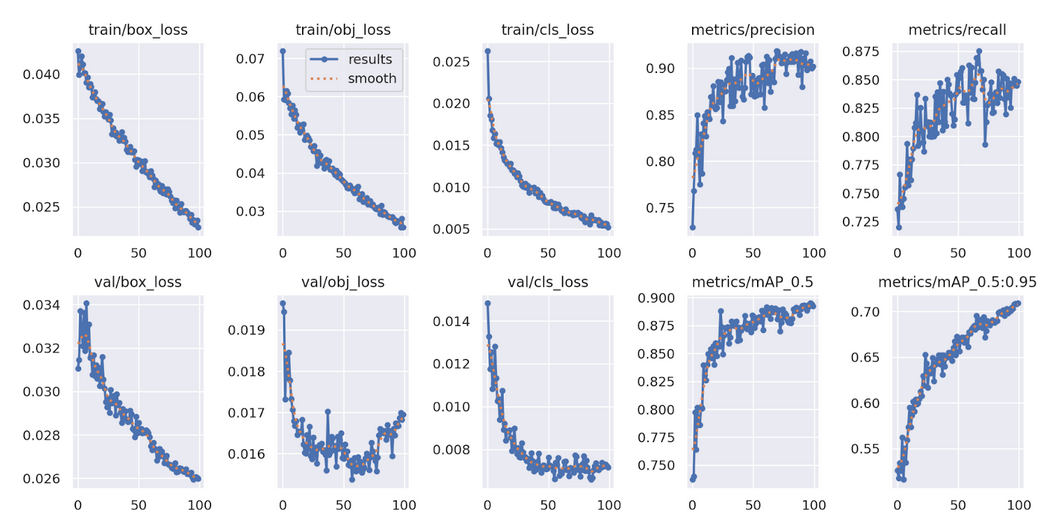
\includegraphics[width=\linewidth,scale=0.8]{statistics.png}
	\caption{Graph depicting the loss value and metric progression during training with 100 epochs}
	\label{fig:graph}
\end{figure}
\FloatBarrier

Figure 4.1 shows the statistics of how the data set performed during training. The loss values used in the graph were box loss, objectness loss, and classification loss. These loss values represent the performance of the model during training concerning the ground truth \cite{
Hui_2022}. Box loss refers to the errors in the location and size of the predicted boundaries, objectness or confidence loss measures the probability that an object exists in the region of interest, and classification loss measures how effective the model is in predicting the correct class. The graph shows that as the training progresses the loss values followed a downward progression which meant that the model is making fewer errors as training continues for both the train and validation sets.

For the metric values there is precision, mean average precision, and recall. Recall is a metric that measures the portion of the true values that are predicted true while precision measures the portion of the predicted values that are true \cite{D_Powers}. Mean average precision was calculated by averaging the precision of each class and then averaging all the precision of every class \cite{Shah_2022}. In the graph, the metrics show an upward, although not linear, progression along 100 epochs, which means that the model is improving continuously for training and validation. 
 

\subsection{Confusion Matrix/F-1 Score Calculation}
After training the model, a confusion matrix was provided (figure \ref{fig:con_mat}) which depicts the normalized count of predicted versus true values of the six (6) classes and the background in the model, and is useful for getting the metrics necessary to measure the performance of the model.
The normalization of the confusion matrix was obtained by dividing each of the row's elements to the sum of the entire row. The normalized elements all add up to 1.0. This allows the matrix to be read in percentages.

The diagonal boxes (which are dark blue in figure \ref{fig:con_mat})indicate the true positives, wherein the predicted vehicle during training is actually the proper vehicle type. The true positives of every vehicle all have a good score, with tricycles having the highest value of 0.90 or 90\% accurately detected as tricycles. 

The columns, excluding the diagonal elements (dark blue) of true positives, indicate the false negatives. These are instances where the vehicle was detected as another type (i.e. 1\% of cars were detected as either a jeepney, motorcycle, or utility vehicle).

The "background" class was included for the instance where the detected object is anything but vehicle. The background row signifies the percentages of the vehicles not being detected. Meanwhile, the background column signifies the instances where a vehicle was detected but in actuality, the detected object is part of the background or is not a vehicle. The background does not have true positive as it is not part of the training process.


 The confusion matrix was made using the validation set of the training data with a confidence of 0.25 based on the source code of YOLOv5. This might cause discrepancies when running the model with real-world data as the confidence value might vary. 


\begin{figure}[!htbp]
	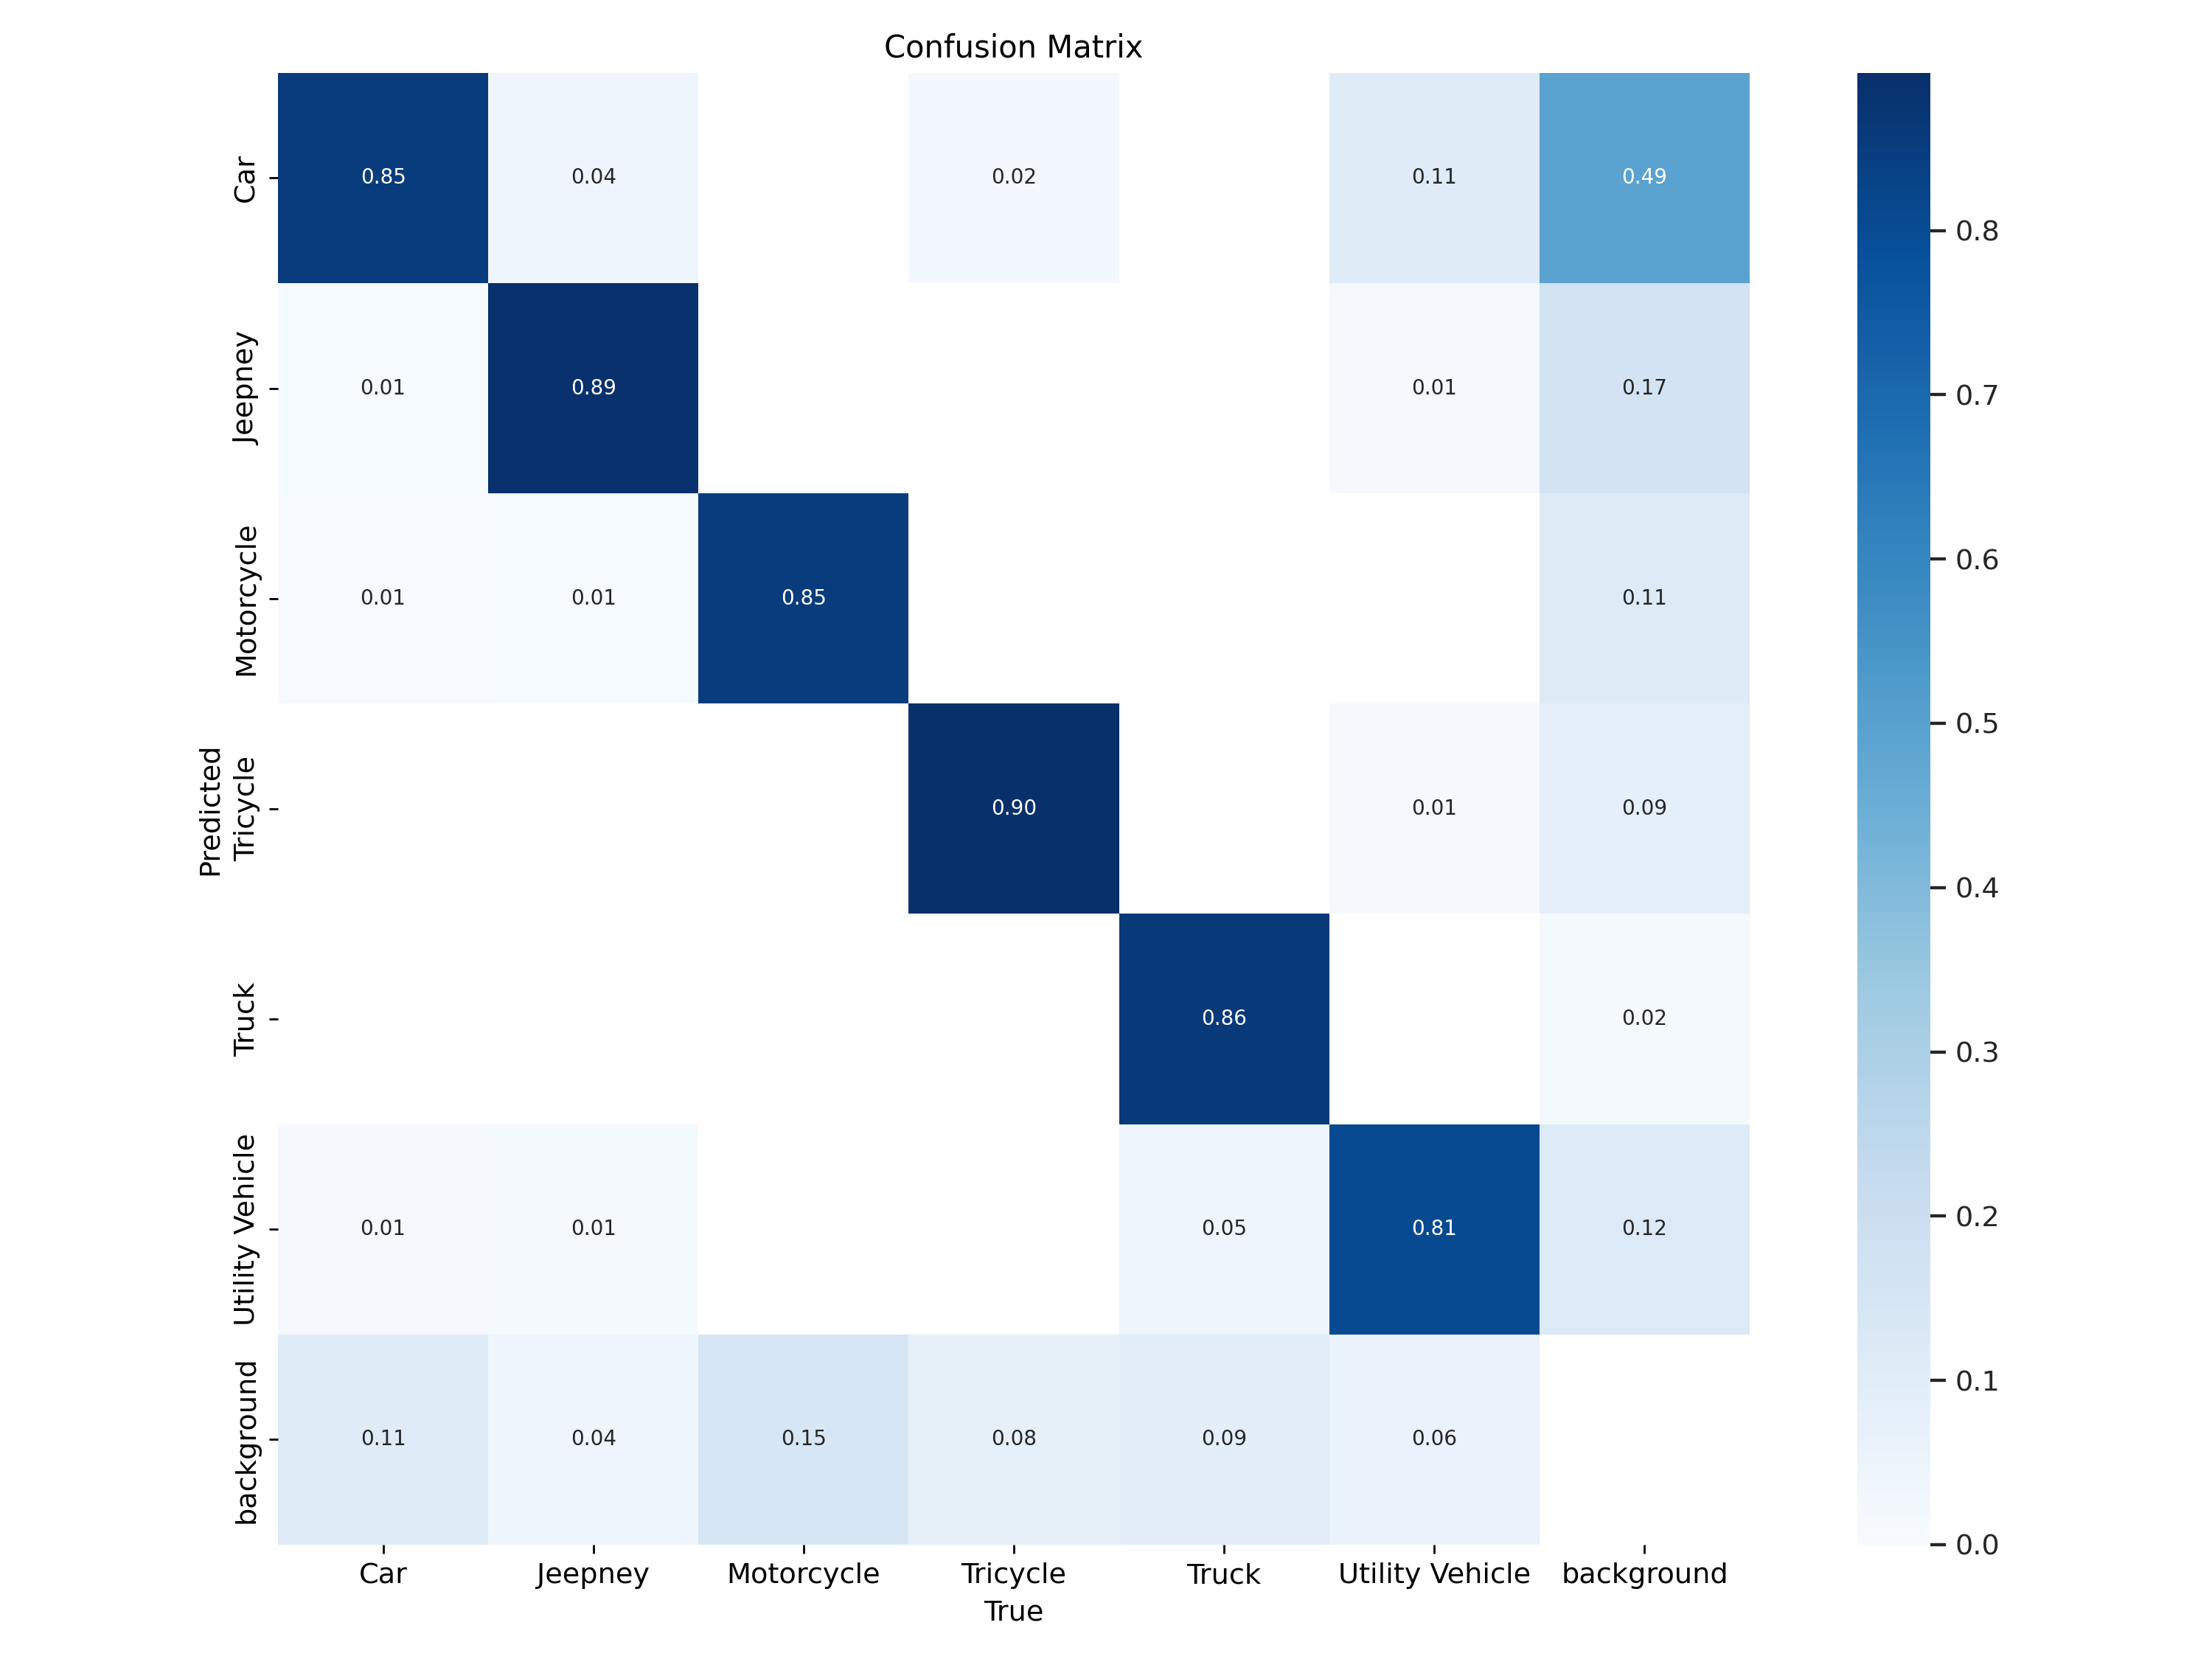
\includegraphics[width=\linewidth,scale=0.8]{confusion_matrix.png}
	\caption{Confusion matrix of the training}
	\label{fig:con_mat}
\end{figure}
\FloatBarrier

For this system, the F1-score metric was used because there was a class imbalance due to the limitations of the locations where the data was taken as shown in Figure \ref{fig:class_bal}. F1-score is a better metric to use compared to accuracy when there is a class imbalance because it measures using the number and type of errors, unlike accuracy which only calculated the number of correct predictions \cite{Korstanje_2021}. Furthermore, the researchers decided that accuracy is not an ideal metric to represent what the model should be predicting, because as a multi-class object detection model that relies on the exact number of vehicles to calculate for emission, it is important to take into account not only the number of correct predictions but also the type of errors, which is what the F1-score metric provides. However, for comparison, the macro averages of the accuracy metric and F1-score metric will be calculated.  

\begin{figure}[!htbp]
	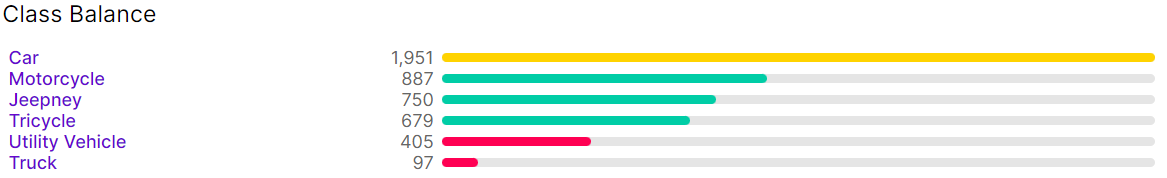
\includegraphics[width=\linewidth,scale=0.8]{class_balance.png}
	\caption{Graph of class balance}
	\label{fig:class_bal}
\end{figure}
\FloatBarrier


To get the F1-score for multi-class classification must be calculated first with the following formulas which were taken from the Towards Data Science article \cite{Korstanje_2021} and from Powers \citeyear{D_Powers}:

\begin{equation}
	{\text{Accuracy}}= \frac{\text{Correct Predictions}}{\text{Total Predictions}} 
\end{equation}


\begin{equation}
{\text{Precision}}= \frac{\text{class TP}}{\text{class TP}+\text{class FP}} 
\end{equation}

\begin{equation}
{\text{Recall}}= \frac{\text{class TP}}{\text{class TP}+\text{class FN}} 
\end{equation}


\begin{equation}
{\text{F1}}= 2 * \frac{\text{Precision}*\text{Recall}}{\text{Precision}+\text{Recall}} 
\end{equation}


For calculating the precision, we can get the values available in the confusion matrix in Figure 4.1. In the following example, the precision for the “Car” class is calculated using the formula from equation 4.1:

\[{\text{Precision\textsubscript{Car}}}= \frac{0.85}{0.85+(0.04+0+0.02+0+0.11+0.49)} \]

\[{\text{Precision\textsubscript{Car}}}= \frac{0.85}{1.51} \]

\[{\text{Precision\textsubscript{Car}}}= 0.5629139073 \]

The value 0.85 was taken from the cell of the predicted and true value for the “Car” class which means that it is a true positive because the predicted objects were the true objects. The false positives from the matrix are the other classes that are predicted as the “Cars” class in the confusion matrix. Applying the method above but for the recall value of the “Car” class:


\[{\text{Recall\textsubscript{Car}}}= \frac{0.85}{0.85+(0.01+0.01+0+0+0.01+0.11)} \]

\[{\text{Recall\textsubscript{Car}}}= \frac{0.85}{0.99} \]

\[{\text{Recall\textsubscript{Car}}}= 0.8585858586 \]

Similar for the calculation of precision, we get 0.85 as true positive from the confusion matrix. In this case, however, the formula uses false negatives which are classes from the confusion matrix that detected a car for objects that are not cars. Using both precision and recall the F1-score can be calculated by:

\[{\text{F1}\textsubscript{Car}}= 2 * \frac{0.5629139073*0.8585858586}{0.5629139073+0.8585858586} \]

\[{\text{F1}\textsubscript{Car}}= 2 * \frac{0.4833099204}{1.421499766} \]

\[{\text{F1}\textsubscript{Car}}= 2 * 0.34 \]

\[{\text{F1}\textsubscript{Car}}= 0.68 \]

Lastly, to calculate for accuracy the number of true predictions (true positive and true negatives) was divided by all the values in the confusion matrix. Below is the calculation of accuracy for the “Car” class:

\[{\text{Accuracy}\textsubscript{Car}}= \frac{0.85 + 5.33}{6.98} \]

\[{\text{Accuracy}\textsubscript{Car}}=  \frac{6.18}{6.98} \]


\[{\text{Accuracy}\textsubscript{Car}}= 0.8853868195 \]


With this methods, the performance metrics of each class was calculated and the results are shown in Table \ref{tab:perf_mat}. 


\begin{table}[ht]   %t means place on top, replace with b if you want to place at the bottom
	\centering
	\caption{Table of performance metrics of each class} \vspace{0.25em}
	\begin{tabular}{c|c|c|c|c} \hline
		\centering \textbf{Class} & \textbf{Precision} & \textbf{Recall} & \textbf{F1-Score} & \textbf{Accuracy}\\ \hline
		Car & 0.5629139073 & 0.8585858586  & 0.68 & 0.8853868195 \\ \hline
		Jeepney & 0.8240740741 & 0.898989899  & 0.8599033816 & 0.9584527221\\ \hline
		Motorcycle& 0.8673469388  & 0.85   & 0.8585858586 & 0.9598853868 \\ \hline
		Tricycle   & 0.9   & 0.9 & 0.9 & 0.9713467049\\ \hline
		Truck & 0.9772727273 & 0.86 & 0.914893617 & 0.9770773639 \\ \hline
		Utility & 0.81 & 0.81 & 0.81 & 0.9455587393\\ \hline
		
	\end{tabular}
	\label{tab:perf_mat}
\end{table}


Table \ref{tab:perf_mat} showed the Precision value calculated from each class. In the table the class with the lowest precision is the “Car” class which is also the class with the most samples, this is due to the “Car” class being over-represented in the dataset therefore making the system overfit for that particular class, meaning it might detect a car even though it should be a different object \cite{Raj_2019}. On the contrary, the “Truck” class had the highest precision value of approximately 0.9773, which meant that every time the model detects a truck there is a high chance that the model has predicted true \cite{D_Powers}, even though the “Truck” class was underrepresented in the dataset. This might be because the trucks are sparse in the testing dataset thus making errors rare. Meanwhile, for recall, the “Tricycle” class had the highest value, (0.9) which meant that the model has a high chance of detecting true tricycles in a frame \cite{D_Powers}. Finally, all classes not including the “Car” class had an F1-score of at least 80\%. The “Car” class has an F1-score of 68\%, the lowest of all classes in this model, which was contributed by its low precision value.The accuracy of the model closely follows the ranking of the F1-scores, the only difference is that the ranks of the “Jeepney” and “Motorcycle” classes swapped places for the accuracy metric, also the accuracy of each class was at least 88\%.

To find the overall F1-score of the model the macro average of the F1-scores was used. Macro averages were used instead of micro and weighted averages because macro averages put equal importance on all the classes in the model whereas weighted averages are ideal for datasets with classes having different degrees of importance and micro averages are ideal for datasets with a balanced distribution of classes \cite{Leung_2022}. The Macro averages can be calculated by finding the average of the F1-score and accuracy metric from each class \cite{Leung_2022}. To find the macro average of the F1-score and accuracy the average of their respective column were calculated from Figure 4.3.

Equation:
\begin{equation}
	{\text{metric}}= \frac{\text{sum of all values of the metric}}{\text{number of classes}} 
\end{equation}

For F1-score:

\[{\text{F1}}= \frac{0.68 + 0.8599033816 + 0.8585858586 + 0.9 + 0.914893617 + 0.81}{6} \]

\[{\text{F1}}=  \frac{5.023382857}{6} \]


\[{\text{F1}}= 0.8372304762 \]

For Accuracy:


\[{\text{Accuracy}}= \frac{0.89 + 0.96 + 0.96 + 0.97 + 0.98 + 0.95}{6} \]

\[{\text{Accuracy}}=  \frac{5.70}{6} \]


\[{\text{Accuracy}}= 0.95 \]

The model had an accuracy of approximately 95\% not taking into account the errors it made. However, if the errors were considered the model only has an accuracy of approximately 84\% which is lower but is more ideal for the imbalance distribution of classes in the dataset. Nonetheless, the model was accurate enough to be used for object detection.




\section{Object Detection}

The weights obtained through training were used in pre-recorded videos to determine if the weights were trained successfully and to see how they perform in actual video footage. The following locations were chosen by the researchers to be used for the study: Valeria St. , De Leon St., Diversion Road, Lacson St., Roxas Ave. The locations were chosen for their variety in vehicle congestion and vehicle type (i.e. Diversion Road with a higher vehicle count; Roxas with more tricycles).  These recordings were then processed using the custom vehicle detection Python program. The “processing” includes detecting the vehicles; drawing bounding boxes; and calculating and displaying the approximation of the emission of that area. 

Using the trained model,  the following are the results showing the Ha.Zee system detecting vehicles and their respective types, along with the vehicle $PM_{2.5}$ emission tracker displayed on the upper left portion of the frame. The $PM_{2.5}$ value here means the weight of particulate matter of at most 2.5 micrometers in diameter in kilograms for every kilometer. The higher the value for $PM_{2.5}$ the greater the health risk, but the interpretation of the value on the particulate matter and its consequences falls outside the scope of this study.  To validate the detection model of the system, the researchers compared the ground truth of the total vehicles in the frame via manual counting to the detected vehicles. The information on the system’s detected vehicles stored in the CSV file was utilized in this comparison. This section focused on comparing the number of vehicles the system could detect to the actual vehicle count and does not account for the accuracy of identifying the proper vehicle type.

\subsubsection{Valeria St. (MaryMart, Iloilo City)}


\begin{figure}[!htbp]
	\begin{subfigure}{.5\textwidth}
		\centering
		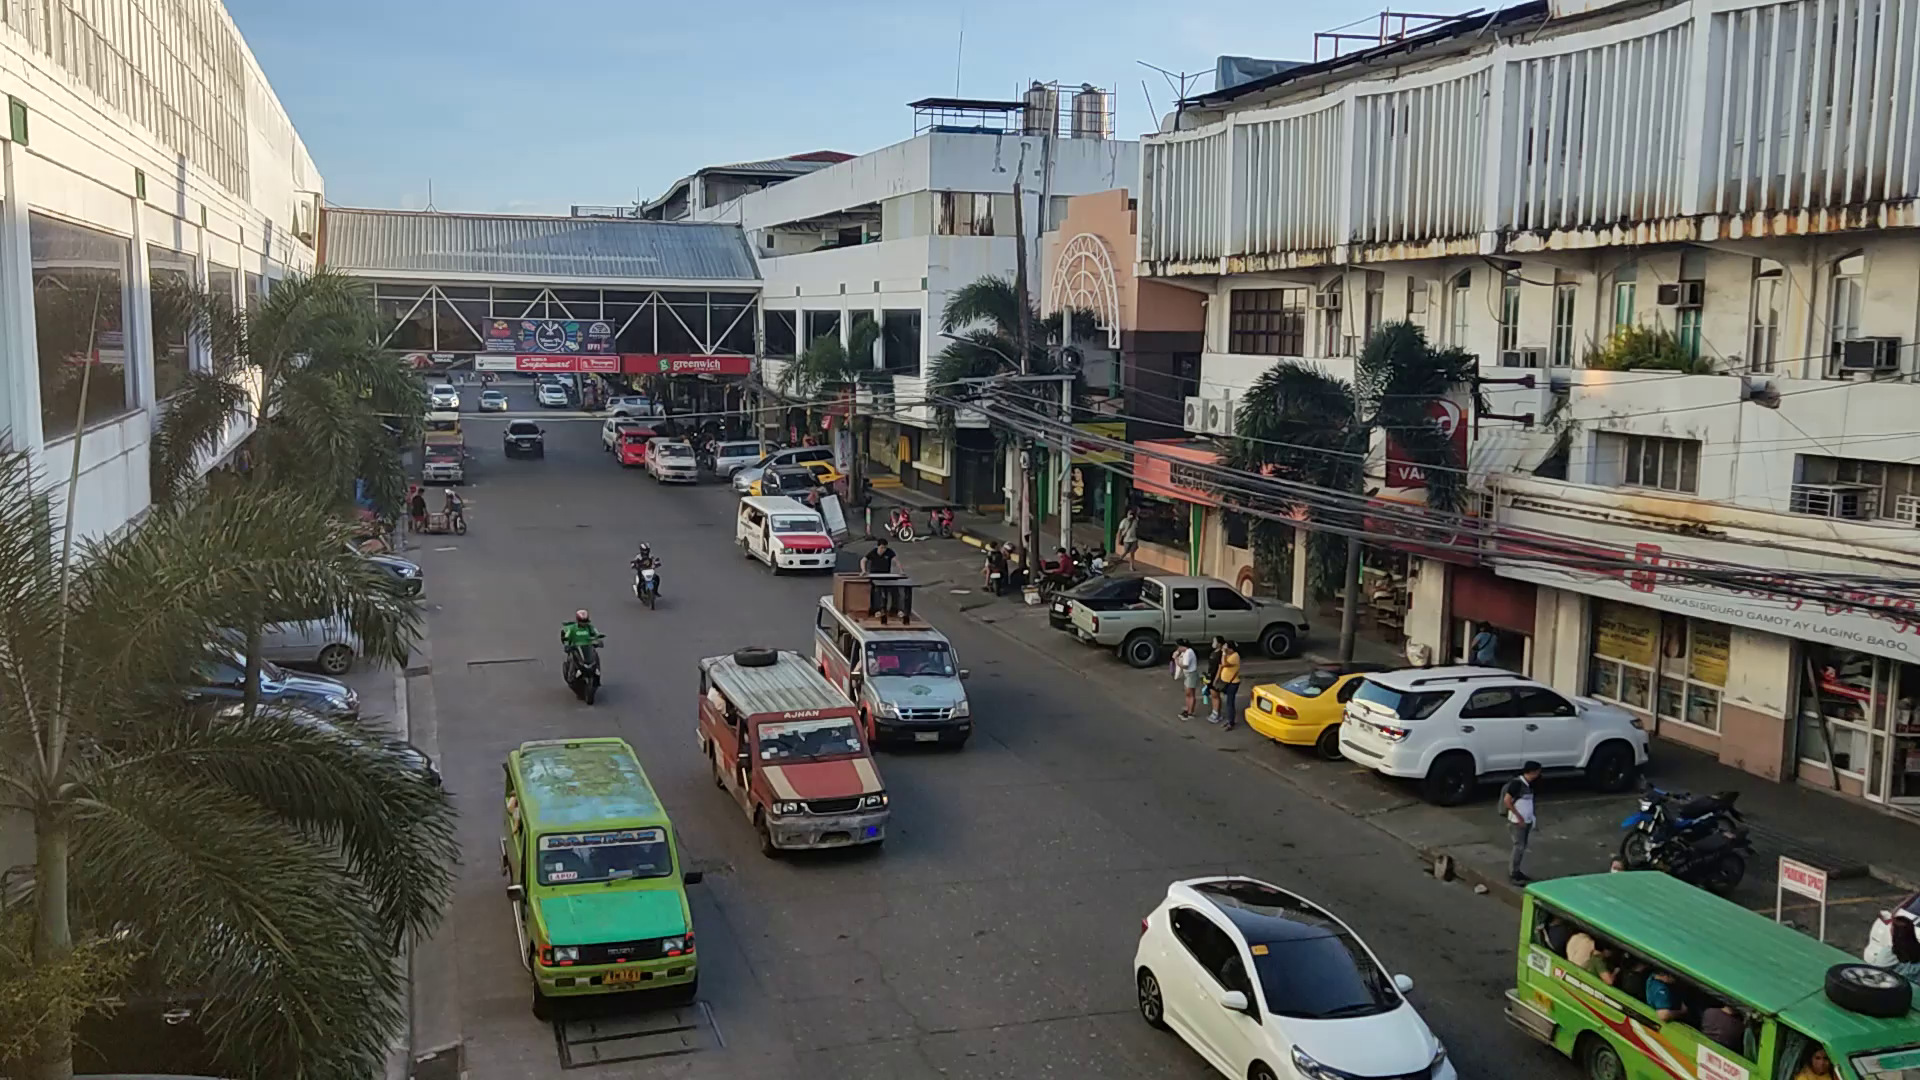
\includegraphics[width=.8\linewidth]{bounding_pics/marymart_unbounded.png}
		\caption{Manual Count: 27 Vehicles}
		
	\end{subfigure}%
	\begin{subfigure}{.5\textwidth}
		\centering
		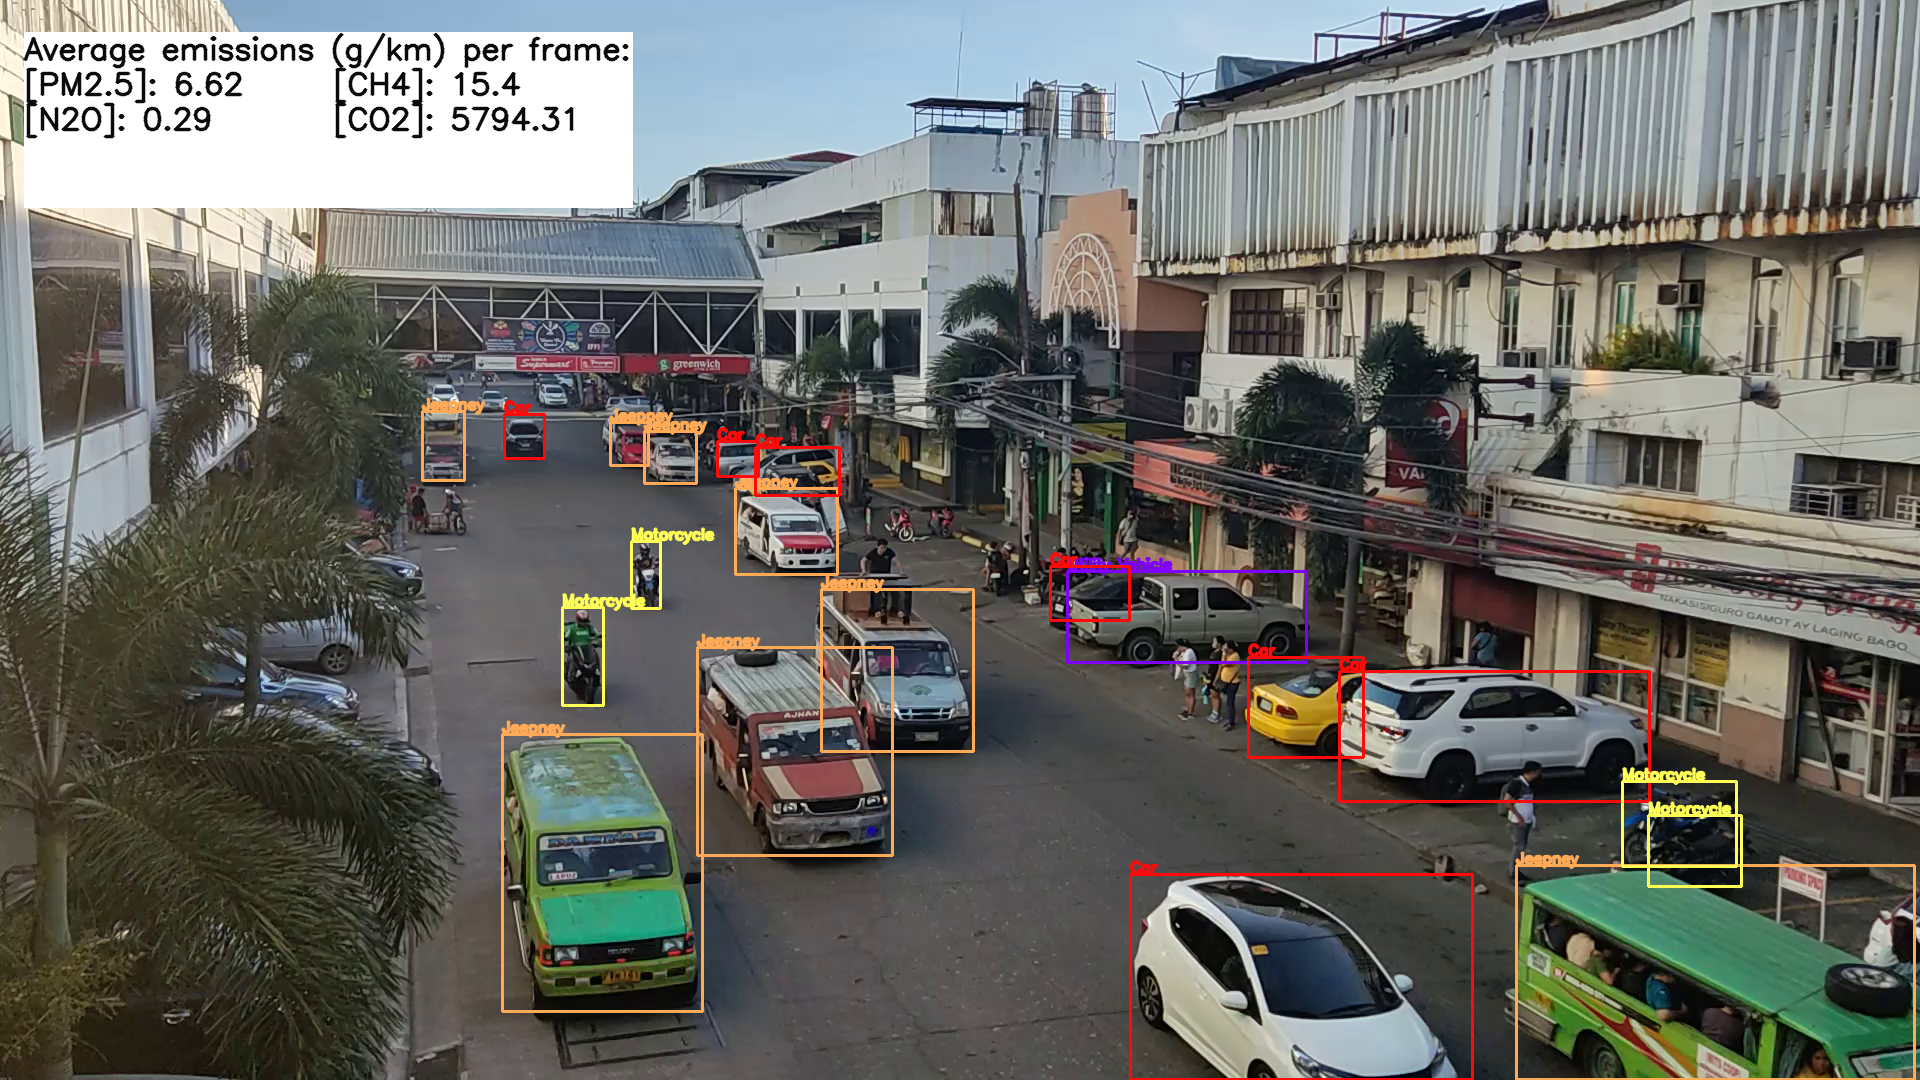
\includegraphics[width=.8\linewidth]{bounding_pics/marymart_bounded.png}
		\caption{Ha.Zee Count: 17 vehicles}
	\end{subfigure}
	\caption{Valeria St. Traffic Video Footage}
\end{figure}
\FloatBarrier

Using the frame above to represent the video footage from Valeria St., Iloilo City Proper; the researchers manually counted 27 total vehicles. The most common vehicle in this frame is the car, with a count of 12. After using the trained model, the system returned a count of 17 vehicles. In this instance, the most common vehicle type detected was the jeepney, with a count of 8. The road being a route for jeepneys could have influenced their frequency in appearance.

The table below shows the average of vehicles present over the course of the video duration. The average of vehicles appearing in the video is obtained through the sum of the average of a vehicle type’s appearance per second. The same process was applied to the vehicles detected by the system. The ratio between the two counts is then calculated. Of the total average of manually-counted vehicles, only 64.98\% were detected by the system. 



\begin{table}[ht]   %t means place on top, replace with b if you want to place at the bottom
	\centering
	\caption{Ratio of Manual vs. Detected average vehicles counted  (Valeria St.)} \vspace{0.25em}
	\begin{tabular}{c|c|c} \hline
		\centering \textbf {Vehicle type} & \textbf{Manual Count Avg.} & \textbf{Ha.Zee Count Avg.} \\ \hline
		Car & 11.72 & 4.55   \\ 
		Jeepney & 9.72 & 8.18  	\\ 
		Motorcycle& 4.55  & 3.55   \\ 
		Tricycle   & 0  & 0.09  \\ 
		UV & 3 & 1.18  \\ 
		Truck & 0 & 0 \\ \hline
		
		\textbf{Total Average} &27 & 9.145\\ \hline
		\textbf{Ratio/Percentage} & \multicolumn{2}{c}{0.6498}  \\ \hline
		
	\end{tabular}
	\label{tab:valeria_st}
\end{table}

\newpage
\subsubsection{De Leon St.  (Robinsons Place, Iloilo City)
}


\begin{figure}[!htbp]
	\begin{subfigure}{.5\textwidth}
		\centering
		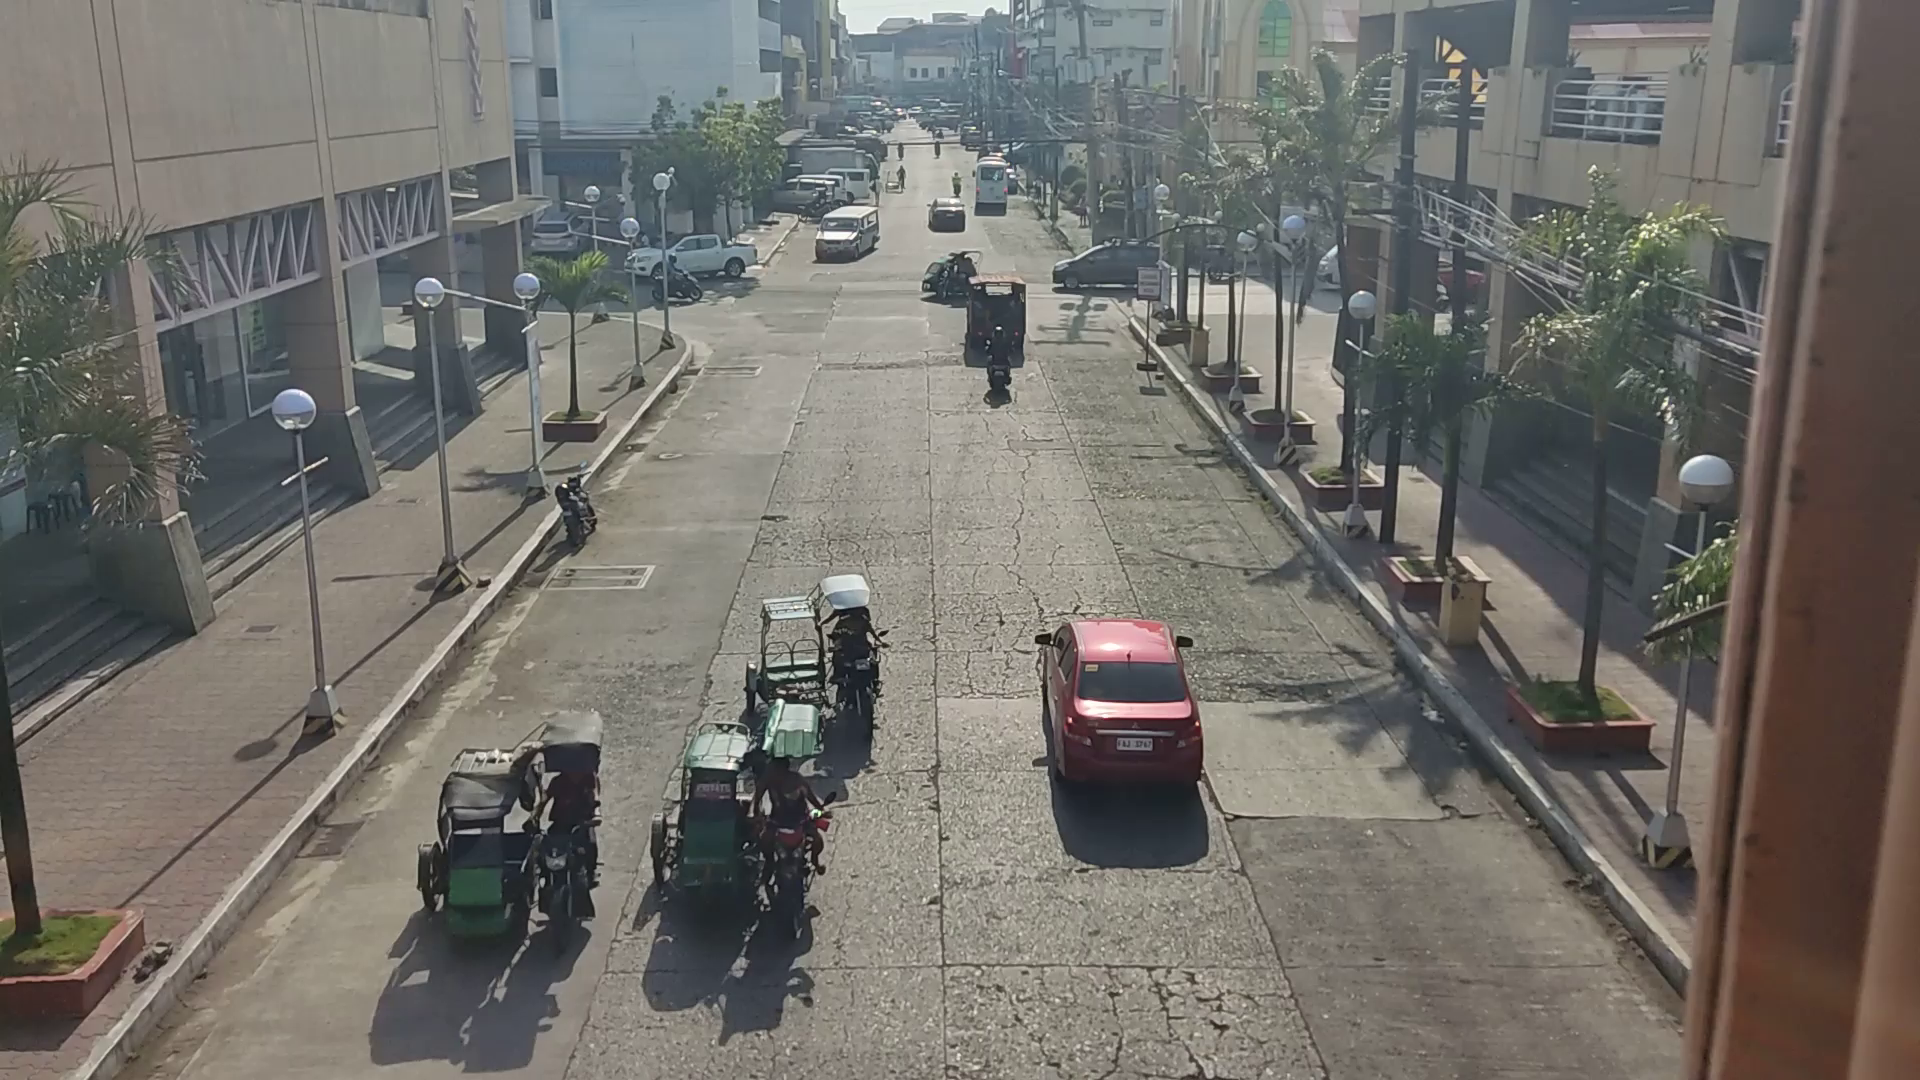
\includegraphics[width=.8\linewidth]{bounding_pics/rob_unbound.png}
		\caption{Manual Count: 15 Vehicles}
		
	\end{subfigure}%
	\begin{subfigure}{.5\textwidth}
		\centering
		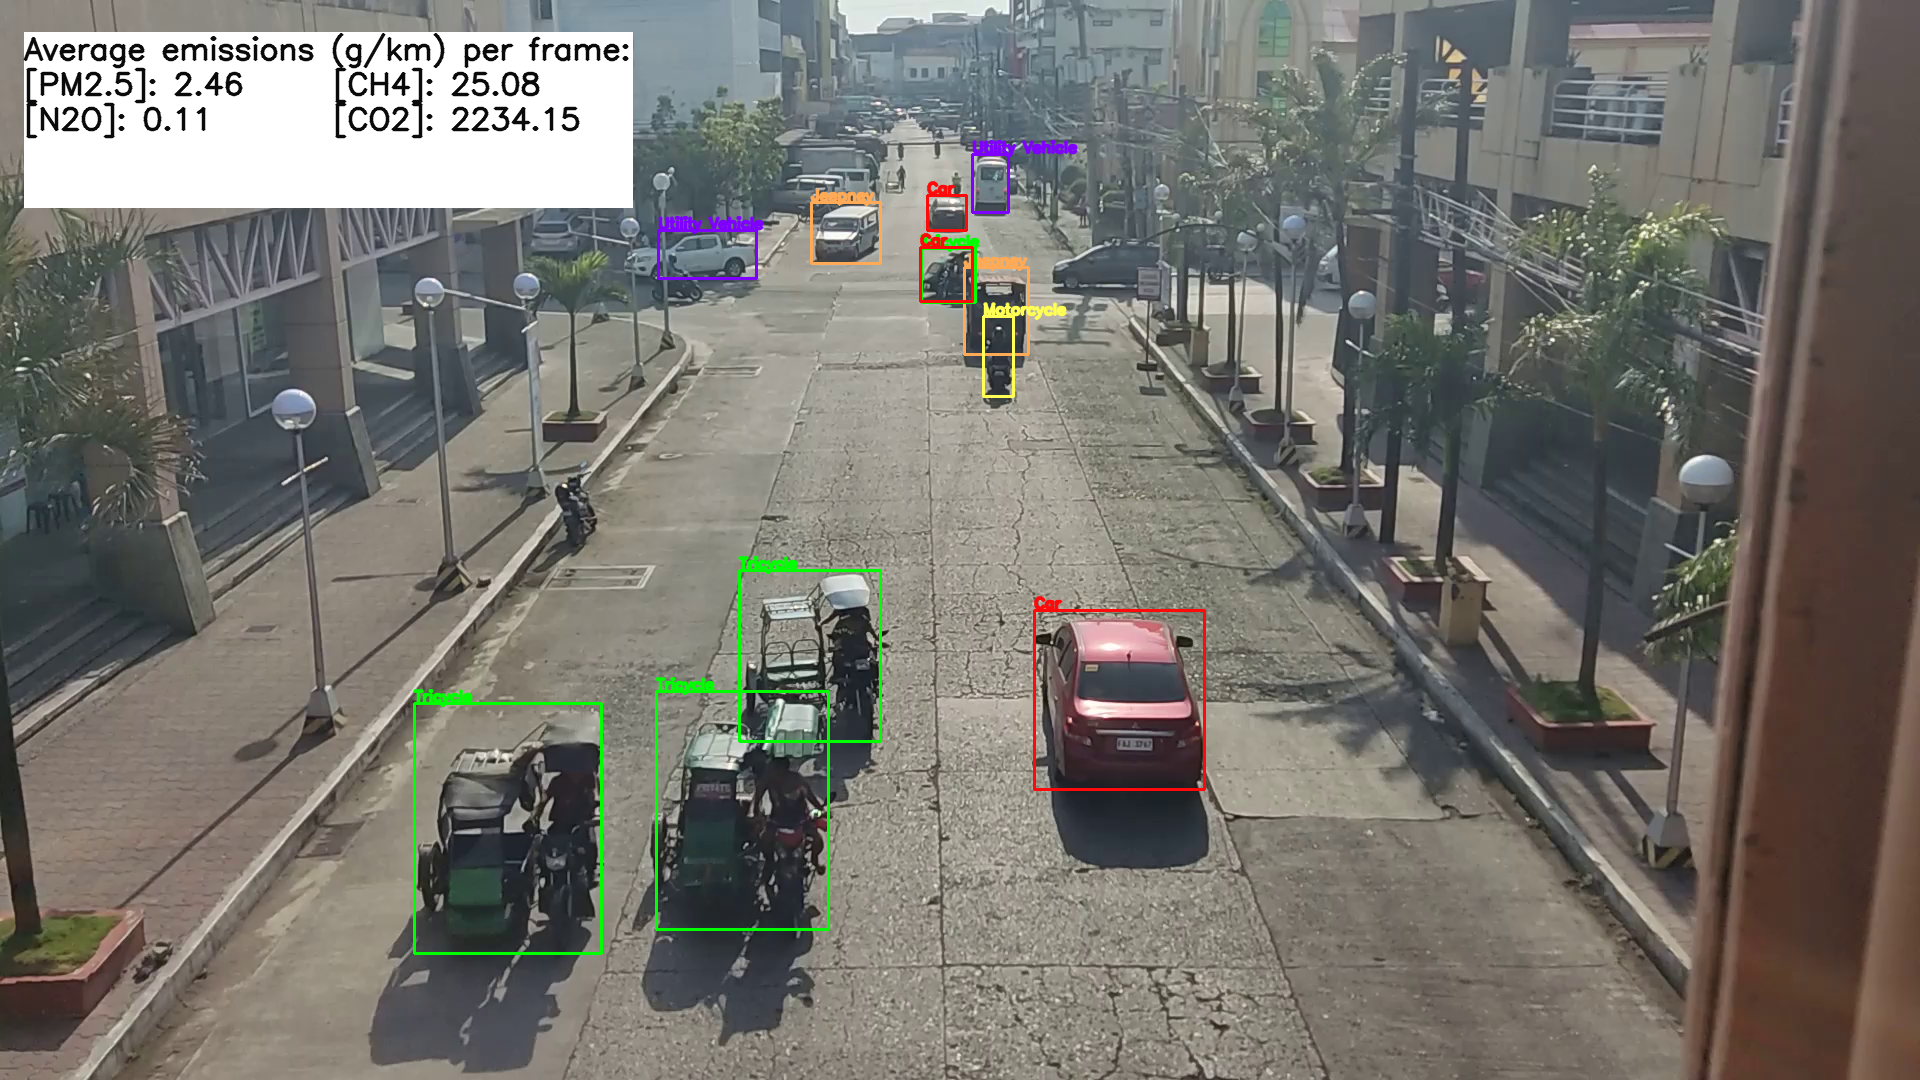
\includegraphics[width=.8\linewidth]{bounding_pics/rob_bound.png}
		\caption{Ha.Zee Count: 10 vehicles}
	\end{subfigure}
	\caption{De Leon St. Traffic Video Footage}
\end{figure}
\FloatBarrier

Using the frame above to represent the video footage from De Leon St., Iloilo City; the researchers manually counted 15 total vehicles. The most common vehicles in this frame are motorcycles and tricycles, both with a count of 4. After using the trained model, the system returned a count of 10 vehicles. In this instance, the most common vehicle type detected was the jeepneys and tricycles, with a count of 3. It is noted that 2 of the detected jeepneys are false positives.

The table below applies the same calculation processes as the previous location. Of the total average of manually-counted vehicles, only 73.28\% were detected by the system. 



\begin{table}[ht]   %t means place on top, replace with b if you want to place at the bottom
	\centering
	\caption{Ratio of Manual vs. Detected average vehicles counted  (De Leon St.)} \vspace{0.25em}
	\begin{tabular}{c|c|c} \hline
		\centering \textbf {Vehicle type} & \textbf{Manual Count Avg.} & \textbf{Ha.Zee Count Avg.}\\ \hline
		Car & 2.63 & 2    \\ 
		Jeepney & 2 & 1.72  	\\ 
		Motorcycle& 3.55  & 1.36  \\ 
		Tricycle   & 3.45  & 3.27  \\ 
		UV & 1.63 & 1.36  \\ 
		Truck & 0 & 0 \\ \hline
		
		\textbf{Total Average} &13.27 & 9.72   \\ \hline
		
		\textbf{Ratio/Percentage} & \multicolumn{2}{c}{0.7328}  \\ \hline
		
	\end{tabular}
	\label{tab:de_leon}
\end{table}

\subsubsection{Diversion Road (Jaro, Iloilo City)
}


\begin{figure}[!htbp]
	\begin{subfigure}{.5\textwidth}
		\centering
		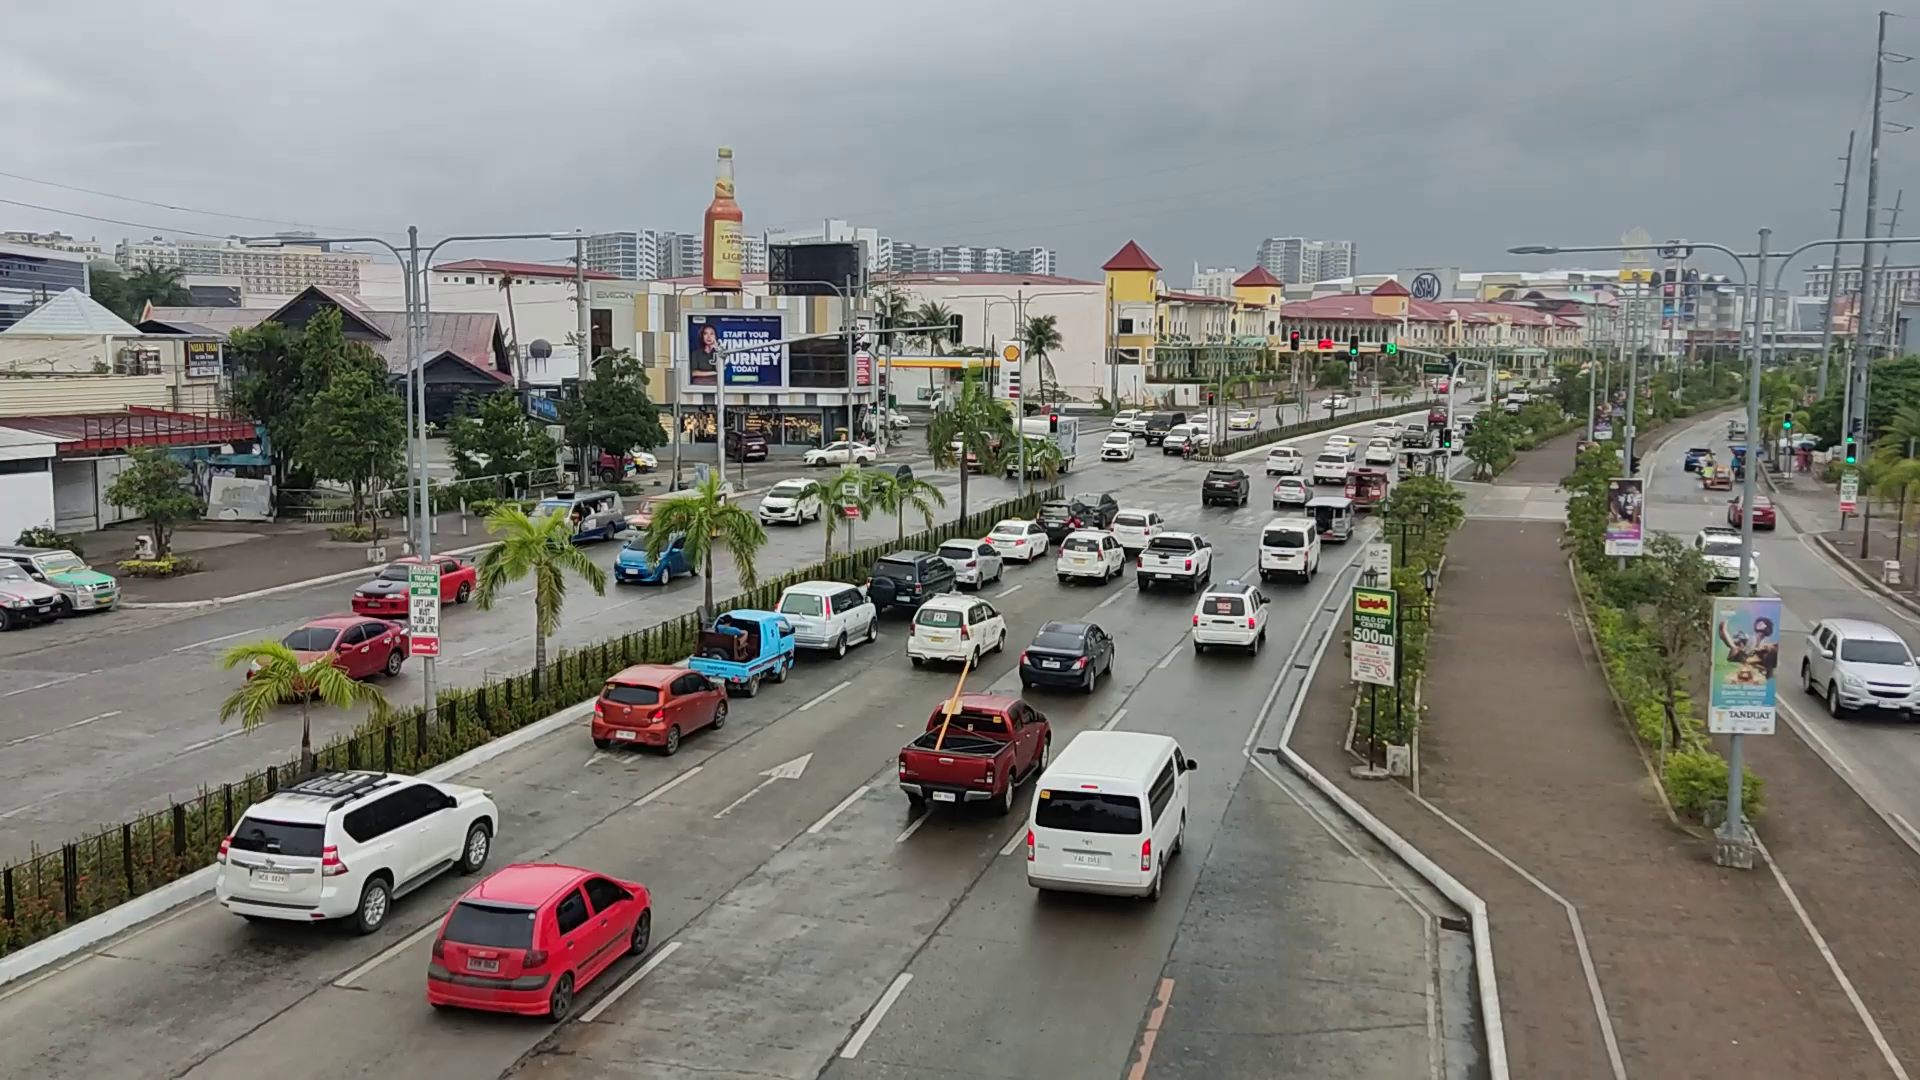
\includegraphics[width=.8\linewidth]{bounding_pics/diversion_unbounded.png}
		\caption{Manual Count: 60 Vehicles}
		
	\end{subfigure}%
	\begin{subfigure}{.5\textwidth}
		\centering
		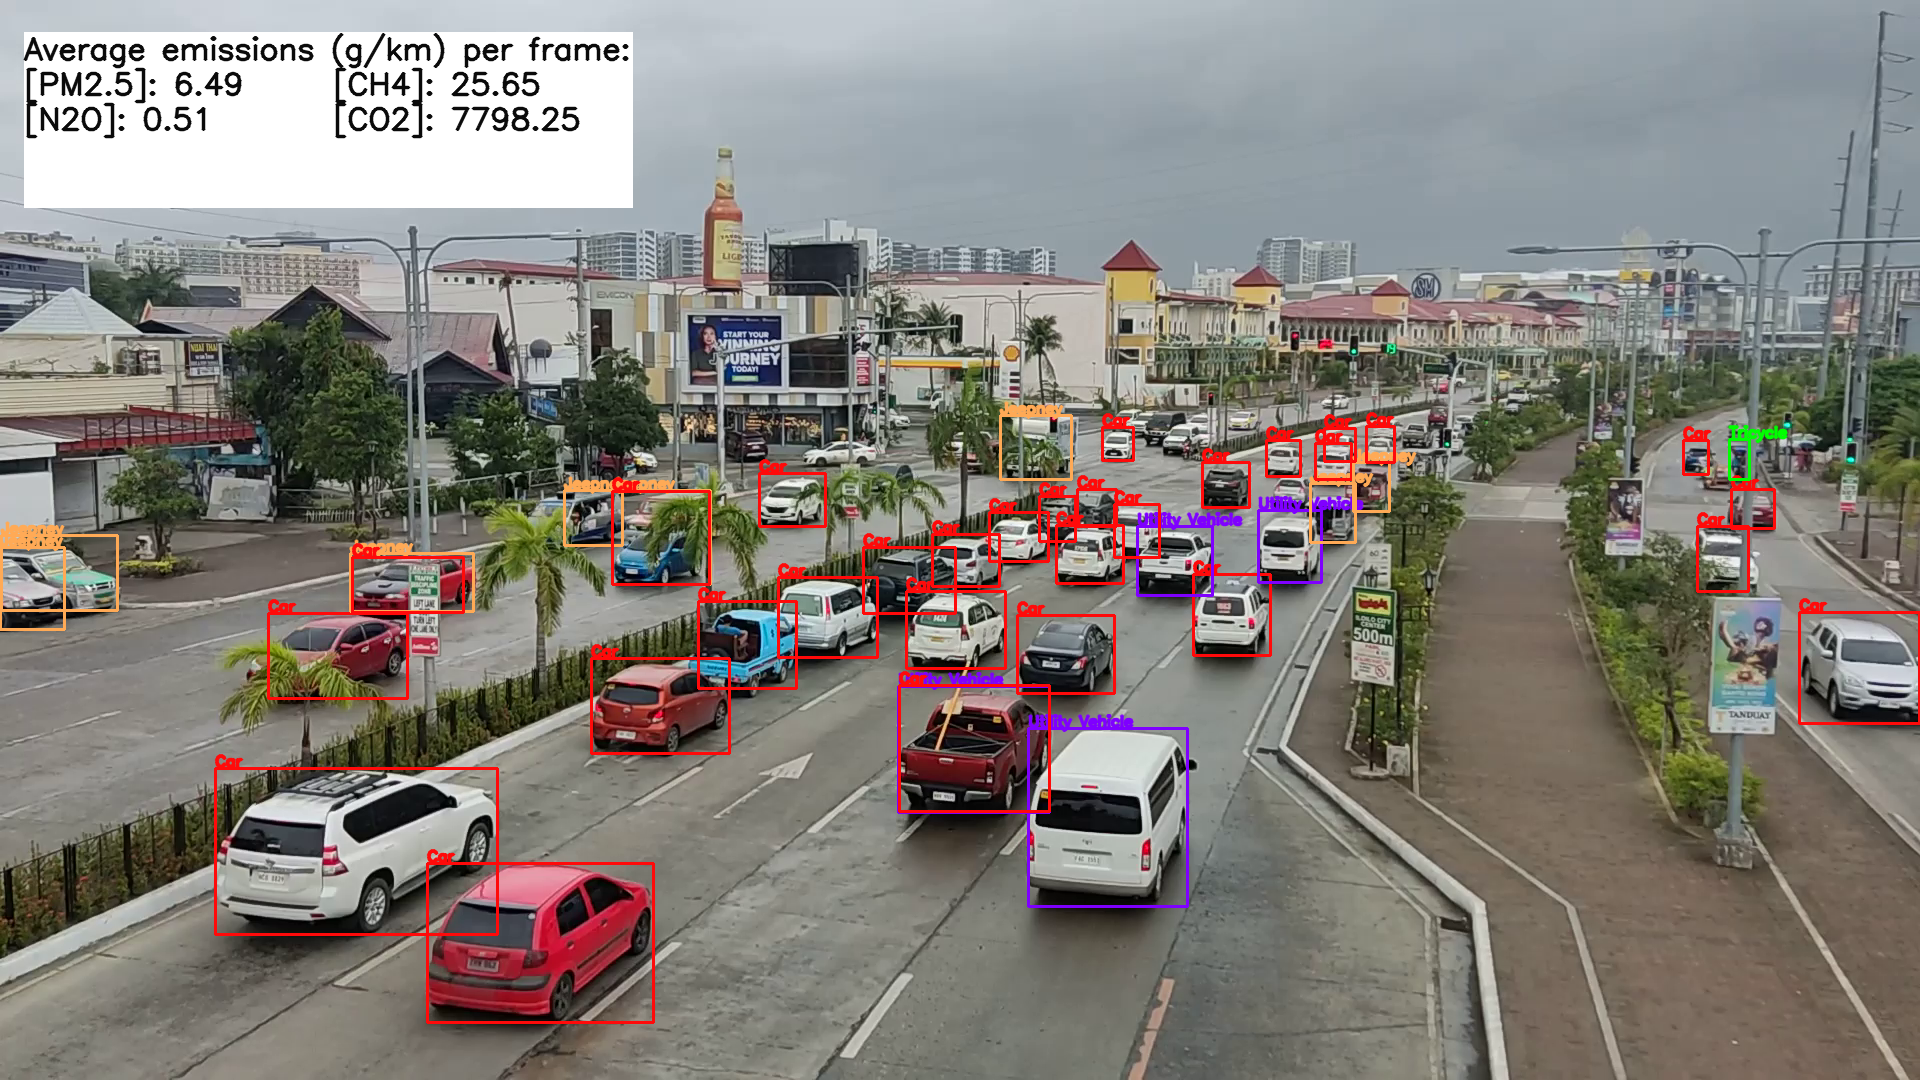
\includegraphics[width=.8\linewidth]{bounding_pics/diversion_bounded.png}
		\caption{Ha.Zee Count: 42 vehicles}
	\end{subfigure}
	\caption{Diversion Road Traffic Video Footage}
\end{figure}
\FloatBarrier

Using the frame above to represent the video footage from Diversion Road, Iloilo City; the researchers manually counted 60 total vehicles. The most common vehicle in this frame is the car, with a count of 46. After using the trained model, the system returned a count of 42 vehicles. In this instance, the most common vehicle type detected was also the car, with a count of 27. Cars are a big majority of this video footage, yet have a big gap in the system’s detection.

The table below applies the same calculation processes as the previous location. Of the total average of manually-counted vehicles, only 71.60\% were detected by the system. 




\begin{table}[ht]   %t means place on top, replace with b if you want to place at the bottom
	\centering
	\caption{Ratio of Manual vs. Detected average vehicles counted  (Diversion Rd.)} \vspace{0.25em}
	\begin{tabular}{c|c|c} \hline
		\centering \textbf {Vehicle type}& \textbf{Manual Count Avg.} & \textbf{Ha.Zee Count Avg.}\\ \hline
		Car & 47.09 & 29.36   \\ 
		Jeepney & 7.90 & 8.09 	\\ 
		Motorcycle& 2.72  & 0.18  \\ 
		Tricycle   & 1.72  & 0.27  \\ 
		UV & 1 & 5.82  \\ 
		Truck & 1 & 0.27 \\ \hline
		
		\textbf{Total Average} & 61.45 & 44\\ \hline
		
		\textbf{Ratio/Percentage} & \multicolumn{2}{c}{0.7160}  \\ \hline
		
	\end{tabular}
	\label{tab:diversion_rd}
\end{table}



\subsubsection{Lacson St. (Bacolod City, Negros Occidental)
}


\begin{figure}[!htbp]
	\begin{subfigure}{.5\textwidth}
		\centering
		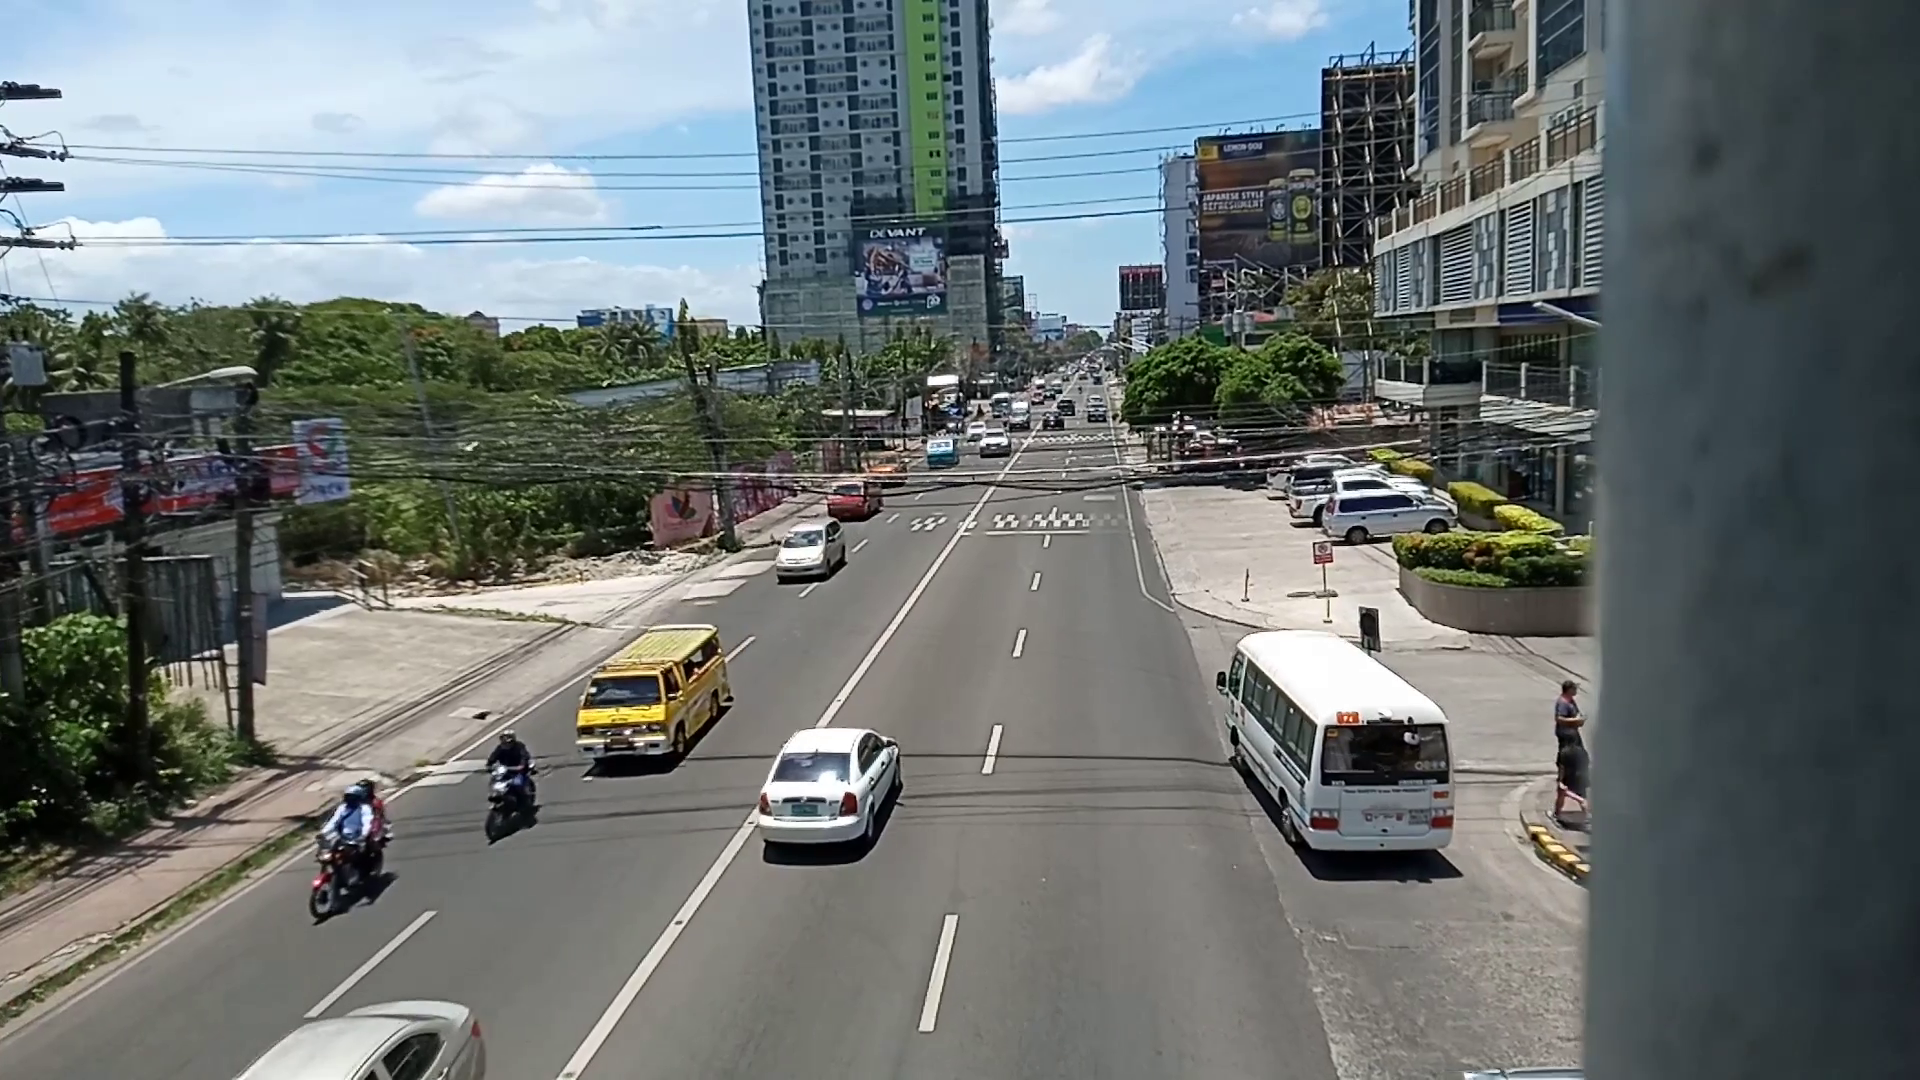
\includegraphics[width=.8\linewidth]{bounding_pics/bacolod_unbound.png}
		\caption{Manual Count: 15 Vehicles}
		
	\end{subfigure}%
	\begin{subfigure}{.5\textwidth}
		\centering
		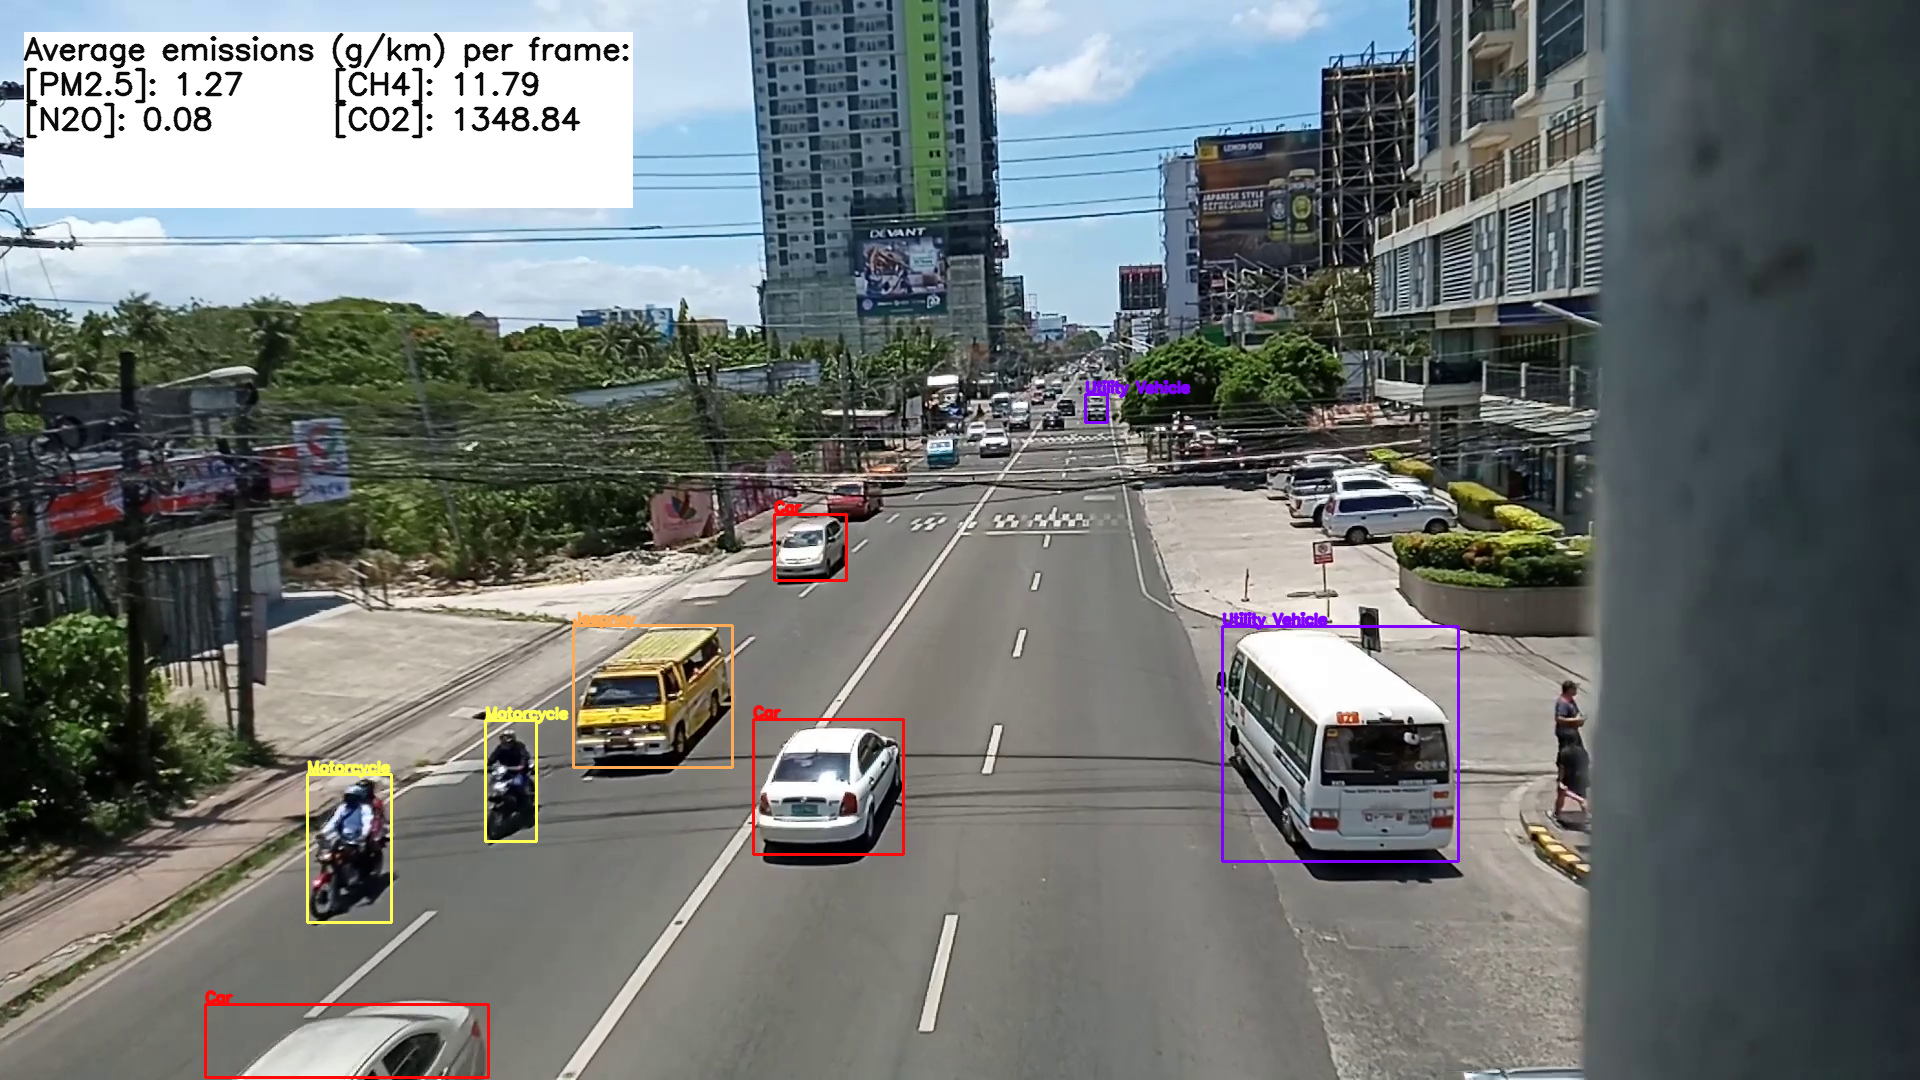
\includegraphics[width=.8\linewidth]{bounding_pics/bacolod_bound.png}
		\caption{Ha.Zee Count: 12 vehicles}
	\end{subfigure}
	\caption{Lacson St. Traffic Video Footage}
\end{figure}
\FloatBarrier

Using the frame above to represent the video footage from Lacson St., Bacolod City; the researchers manually counted 15 total vehicles. The most common vehicle in this frame is the car, with a count of 9. After using the trained model, the system returned a count of 12 vehicles. In this instance, the most common vehicle type detected was also the car, with a count of 5. This being a highway could be the reason why there is a lack of tricycles.

The table below applies the same calculation processes as the previous location. Of the total average of manually-counted vehicles, only 58.42\% were detected by the system. 



\begin{table}[ht]   %t means place on top, replace with b if you want to place at the bottom
	\centering
	\caption{Ratio of Manual vs. Detected average vehicles counted  (Lacson St.)} \vspace{0.25em}
	\begin{tabular}{c|c|c} \hline
		\centering \textbf {Vehicle type} & \textbf{Manual Count Avg.} & \textbf{Ha.Zee Count Avg.} \\ \hline
		Car & 10.45 & 3.18   \\ 
		Jeepney & 2.45 & 1.91  	\\ 
		Motorcycle& 2.27  & 2.09  \\ 
		Tricycle   & 0  & 0.09  \\ 
		UV & 1 & 2.18  \\ 
		Truck & 0 & 0 \\ \hline
		
		\textbf{Total Average} & 16.18 & 9.45  \\ \hline
		
		\textbf{Ratio/Percentage} & \multicolumn{2}{c}{0.5842}  \\ \hline
		
	\end{tabular}
	\label{tab:lacson_st}
\end{table}

\subsubsection{Roxas Ave. (Roxas City, Capiz)
}


\begin{figure}[!htbp]
	\begin{subfigure}{.5\textwidth}
		\centering
		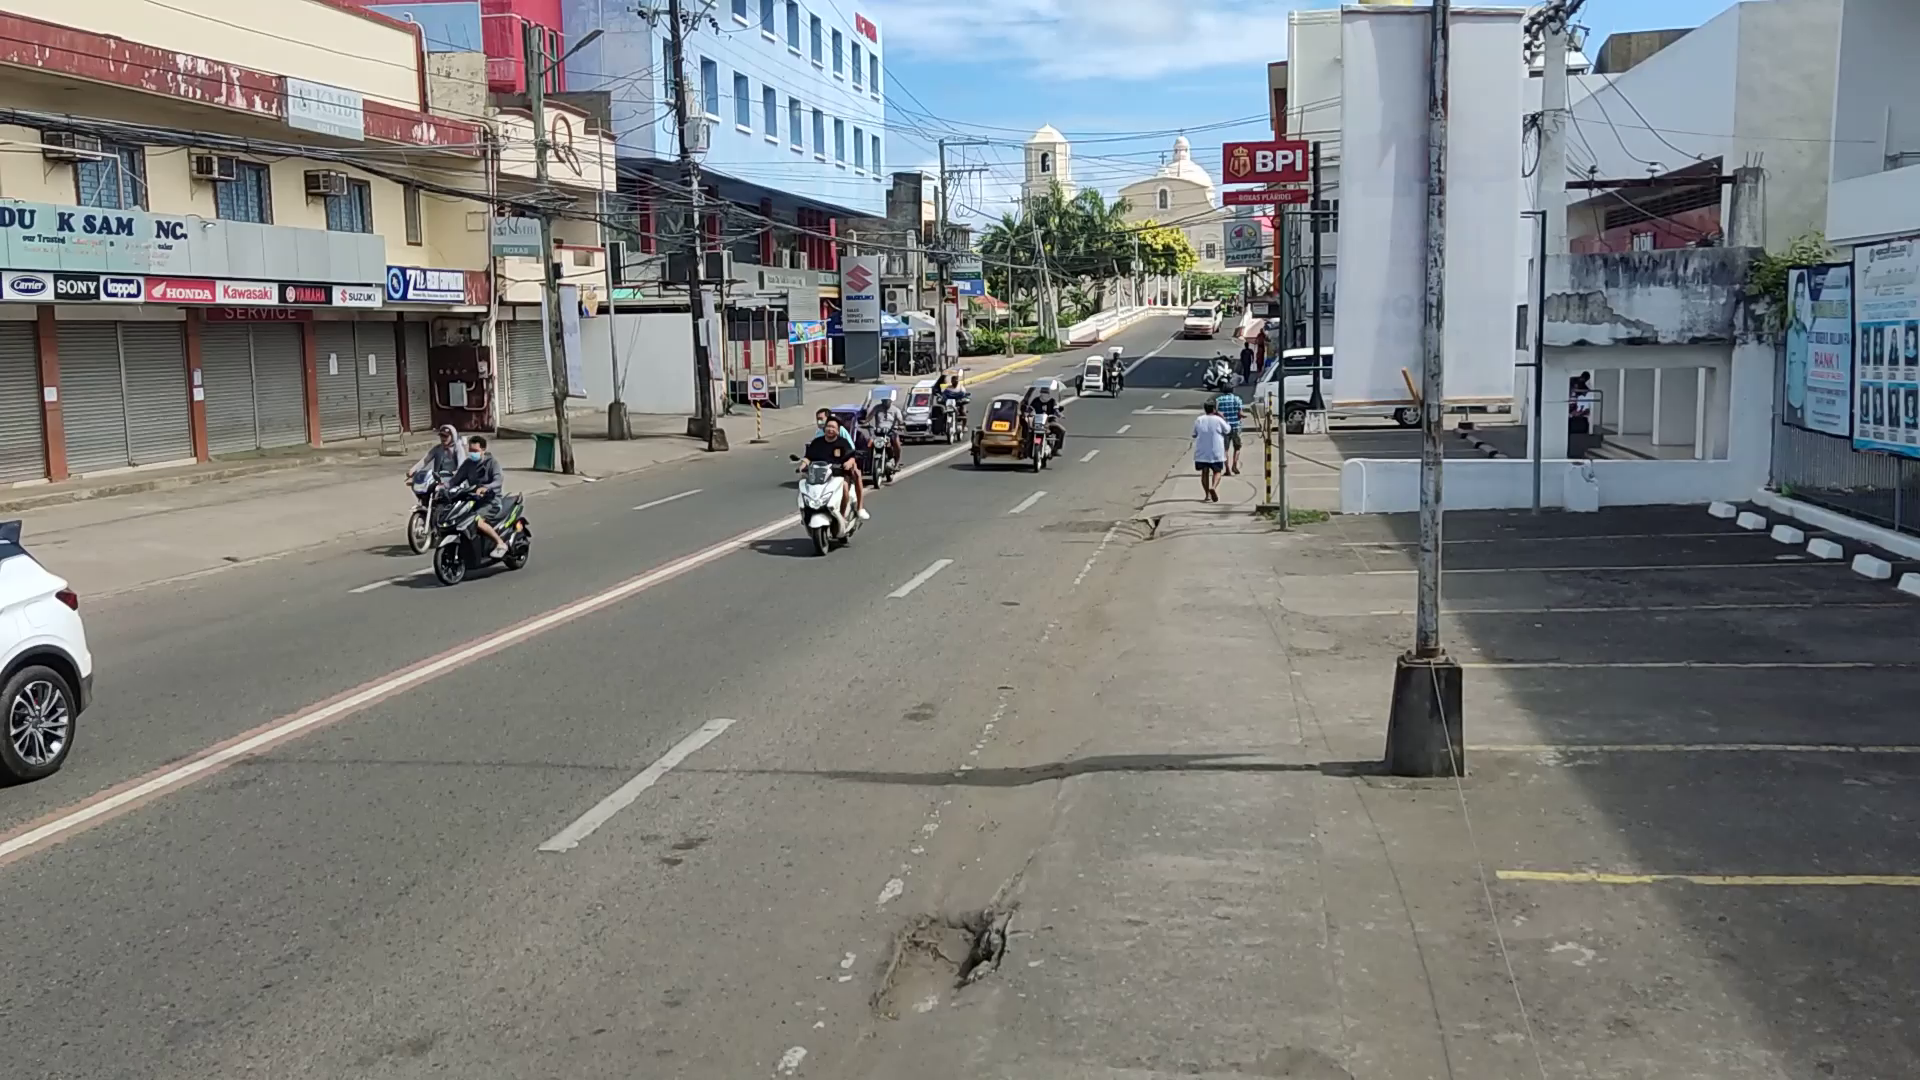
\includegraphics[width=.8\linewidth]{bounding_pics/roxas_unbound.png}
		\caption{Manual Count: 10 Vehicles}
		
	\end{subfigure}%
	\begin{subfigure}{.5\textwidth}
		\centering
		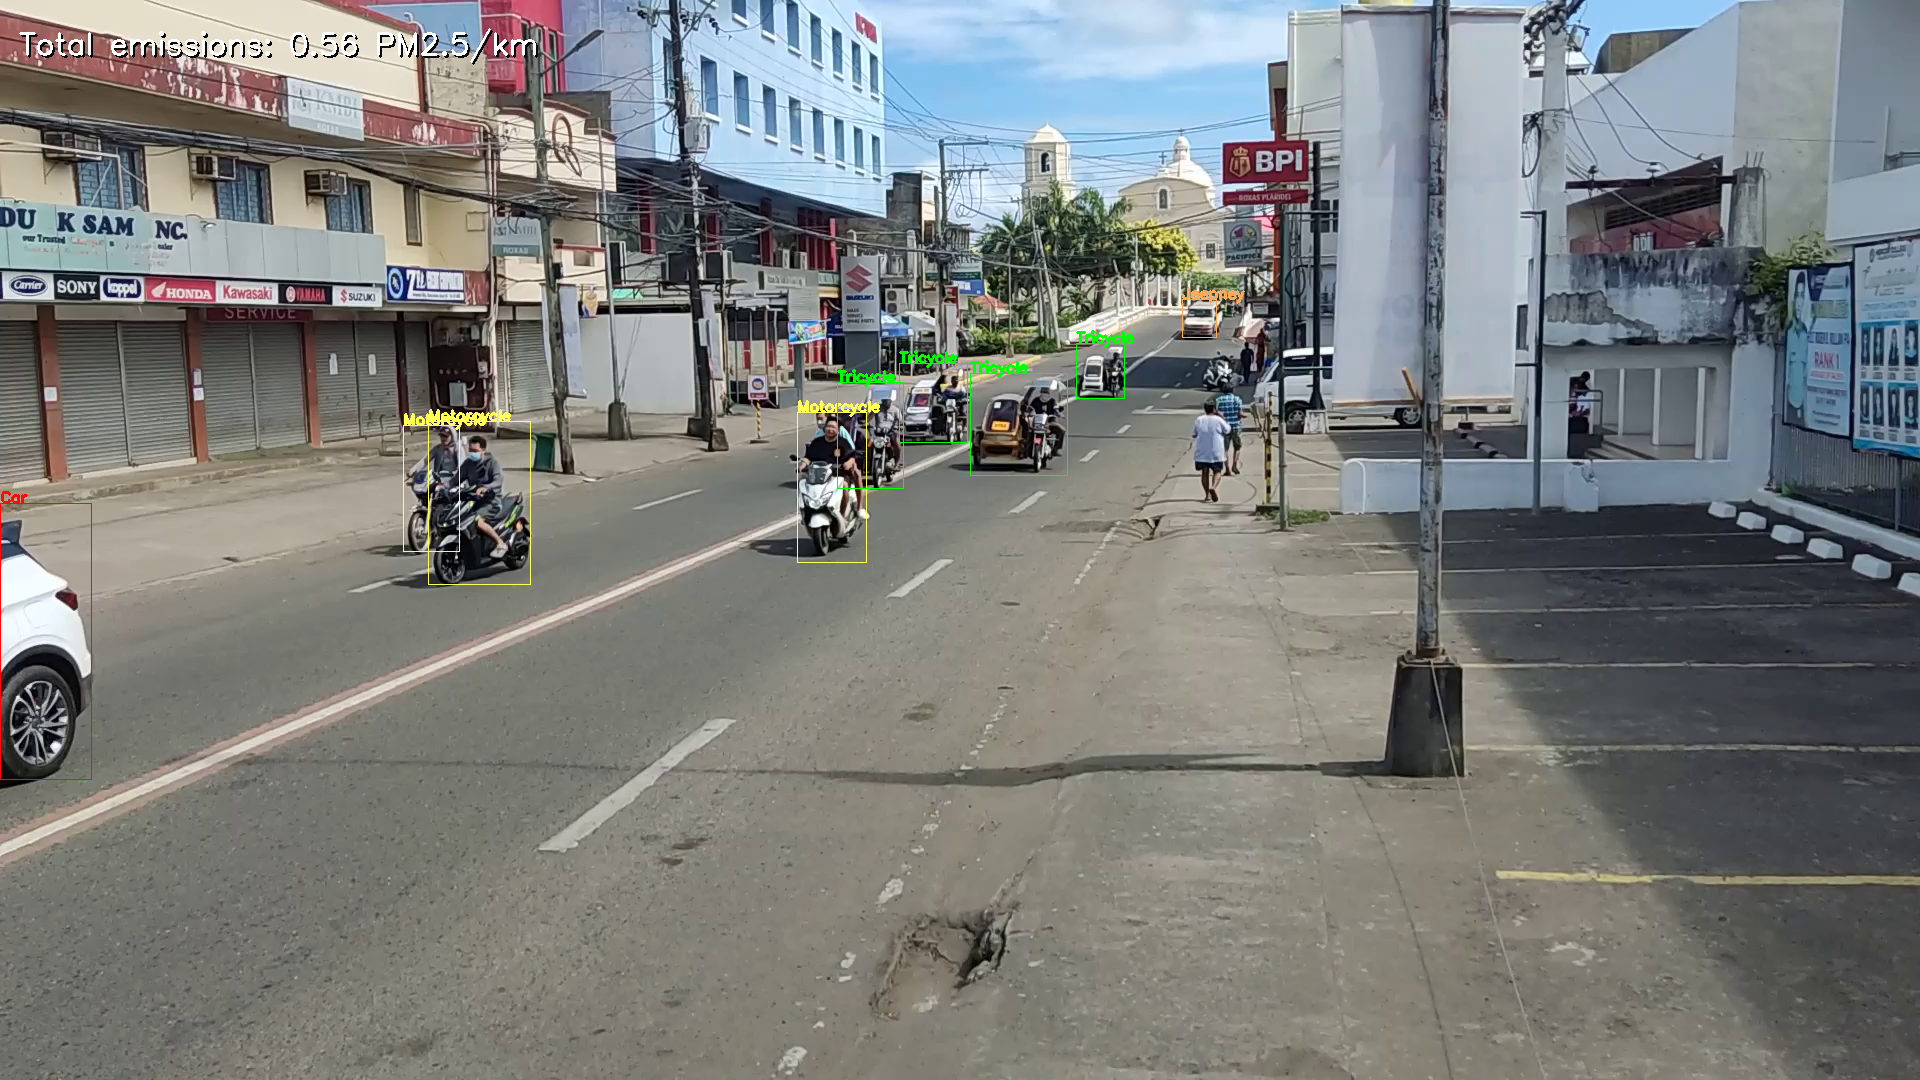
\includegraphics[width=.8\linewidth]{bounding_pics/roxas_bound.png}
		\caption{Ha.Zee Count: 9 vehicles}
	\end{subfigure}
	\caption{Lacson St. Traffic Video Footage}
\end{figure}
\FloatBarrier

Using the frame above to represent the video footage from  Roxas Ave., Roxas City; the researchers manually counted 10 total vehicles. The most common vehicle in this frame is the tricycle, with a count of 4. After using the trained model, the system returned a count of 9 vehicles. In this instance, the most common vehicle type detected was also the tricycles, with the same count of 4. The high count of Tricycles is due to it being one of the main modes of transportation.

The table below applies the same calculation processes as the previous location. Of the total average of manually-counted vehicles, only 77.89\% were detected by the system. 



\begin{table}[ht]   %t means place on top, replace with b if you want to place at the bottom
	\centering
	\caption{Ratio of Manual vs. Detected average vehicles counted  (Roxas Ave.)} \vspace{0.25em}
	\begin{tabular}{c|c|c} \hline
		\centering \textbf {Vehicle type} & \textbf{Manual Count Avg.} & \textbf{Ha.Zee Count Avg.} \\ \hline
		Car & 0.90 & 0.54   \\ \hline
		Jeepney & 0.63 & 0.64  	\\ \hline
		Motorcycle& 2.64  & 1.63  \\ \hline
		Tricycle   & 4.45  & 3.72 \\ \hline
		UV & 0 & 0.18  \\ \hline
		Truck & 0 & 0 \\ \hline
		
		\textbf{Total Average} & 8.63 & 6.73 \\ \hline
		\textbf{Ratio/Percentage} & \multicolumn{2}{c}{0.7789}  \\ \hline
		
		
	\end{tabular}
	\label{tab:roxas_ave}
\end{table}

The ratio between of the actual count of the vehicles compared to the amount detected by the system varies between the 5 locations. Roxas Ave., Roxas City’s video footage had the highest percentage of 77.89\%; while Lacson St. in Bacolod City garnered the lowest percentage of 58.42\%. A factor on why Roxas Ave.’s average of vehicles detected is much closer to the average of the actual vehicles manually counted could be due to the fewer vehicles present and their distance from one another. Said distances could have also been the reason why Diversion Road’s detected cars are significantly lesser than the counted vehicles, as some cars were obstructed by other vehicles and are sometimes counted as a singular vehicle. Another factor that affected the percentages could have been the quality of the video footage used in the study. All the footages shown in the figures were taken from the smartphones of the researchers and rendered some vehicles pixelated, which led to some vehicles being indistinguishable to the system. 



\begin{table}[ht]   %t means place on top, replace with b if you want to place at the bottom
	\centering
	\caption{Average Percentage of Ha.Zee-detected Vehicles.} \vspace{0.25em}
	\begin{tabular}{c|c} \hline
		\centering \textbf {Location} & \textbf {Ratio/Percentages} \\ \hline
		Valeria St. & 0.6498 \\
		De Leon St. & 0.7328 	\\ 
		Diversion Road& 0.7160   \\ 
		Lacson St.   & 0.5842  \\ 
		Roxas Ave.  & 0.7789 \\ \hline
		
		\textbf{Total Average} & 0.6923 \\ \hline
		
	\end{tabular}
	\label{tab:avg_perc}
\end{table}


Across the 5 locations, the system is averaged to detect 69.23\% of the vehicles on a given video footage. This is a reasonably acceptable rate and could be improved upon if more data on different vehicles of varying image qualities were to be added to the training of the system.